\section{Scoring \& Evaluation}

\subsection{NCC}

\todo[inline]{NCC: Upside: Easy to create a score from, set a threshold for 'good' then just divide and give stars}
\todo[inline]{NCC: Downside: Small images lead to big score differences for seemingly small image differences}
\todo[inline]{NCC: Downside: Wasn't ranking the images in the same order that a teacher would}
\todo[inline]{NCC: Downside: Doesn't tell a student what they did wrong, just a black box score, is that all that's needed? - NO}

\subsection{HOG}

\todo[inline]{Similar to NCC, slightly more accurate but more intensive to calculate, see Delteil}

\subsection{Image Difference}

If you're handling simple 1 bit images, you can perform a simple image difference which just takes the first image, XOR'd with the second. The result (shown in Figure \cref{fig:crotchet-diff}) is a simple highlighting of the difference between the two.

\begin{figure}[h!]
  \centering
  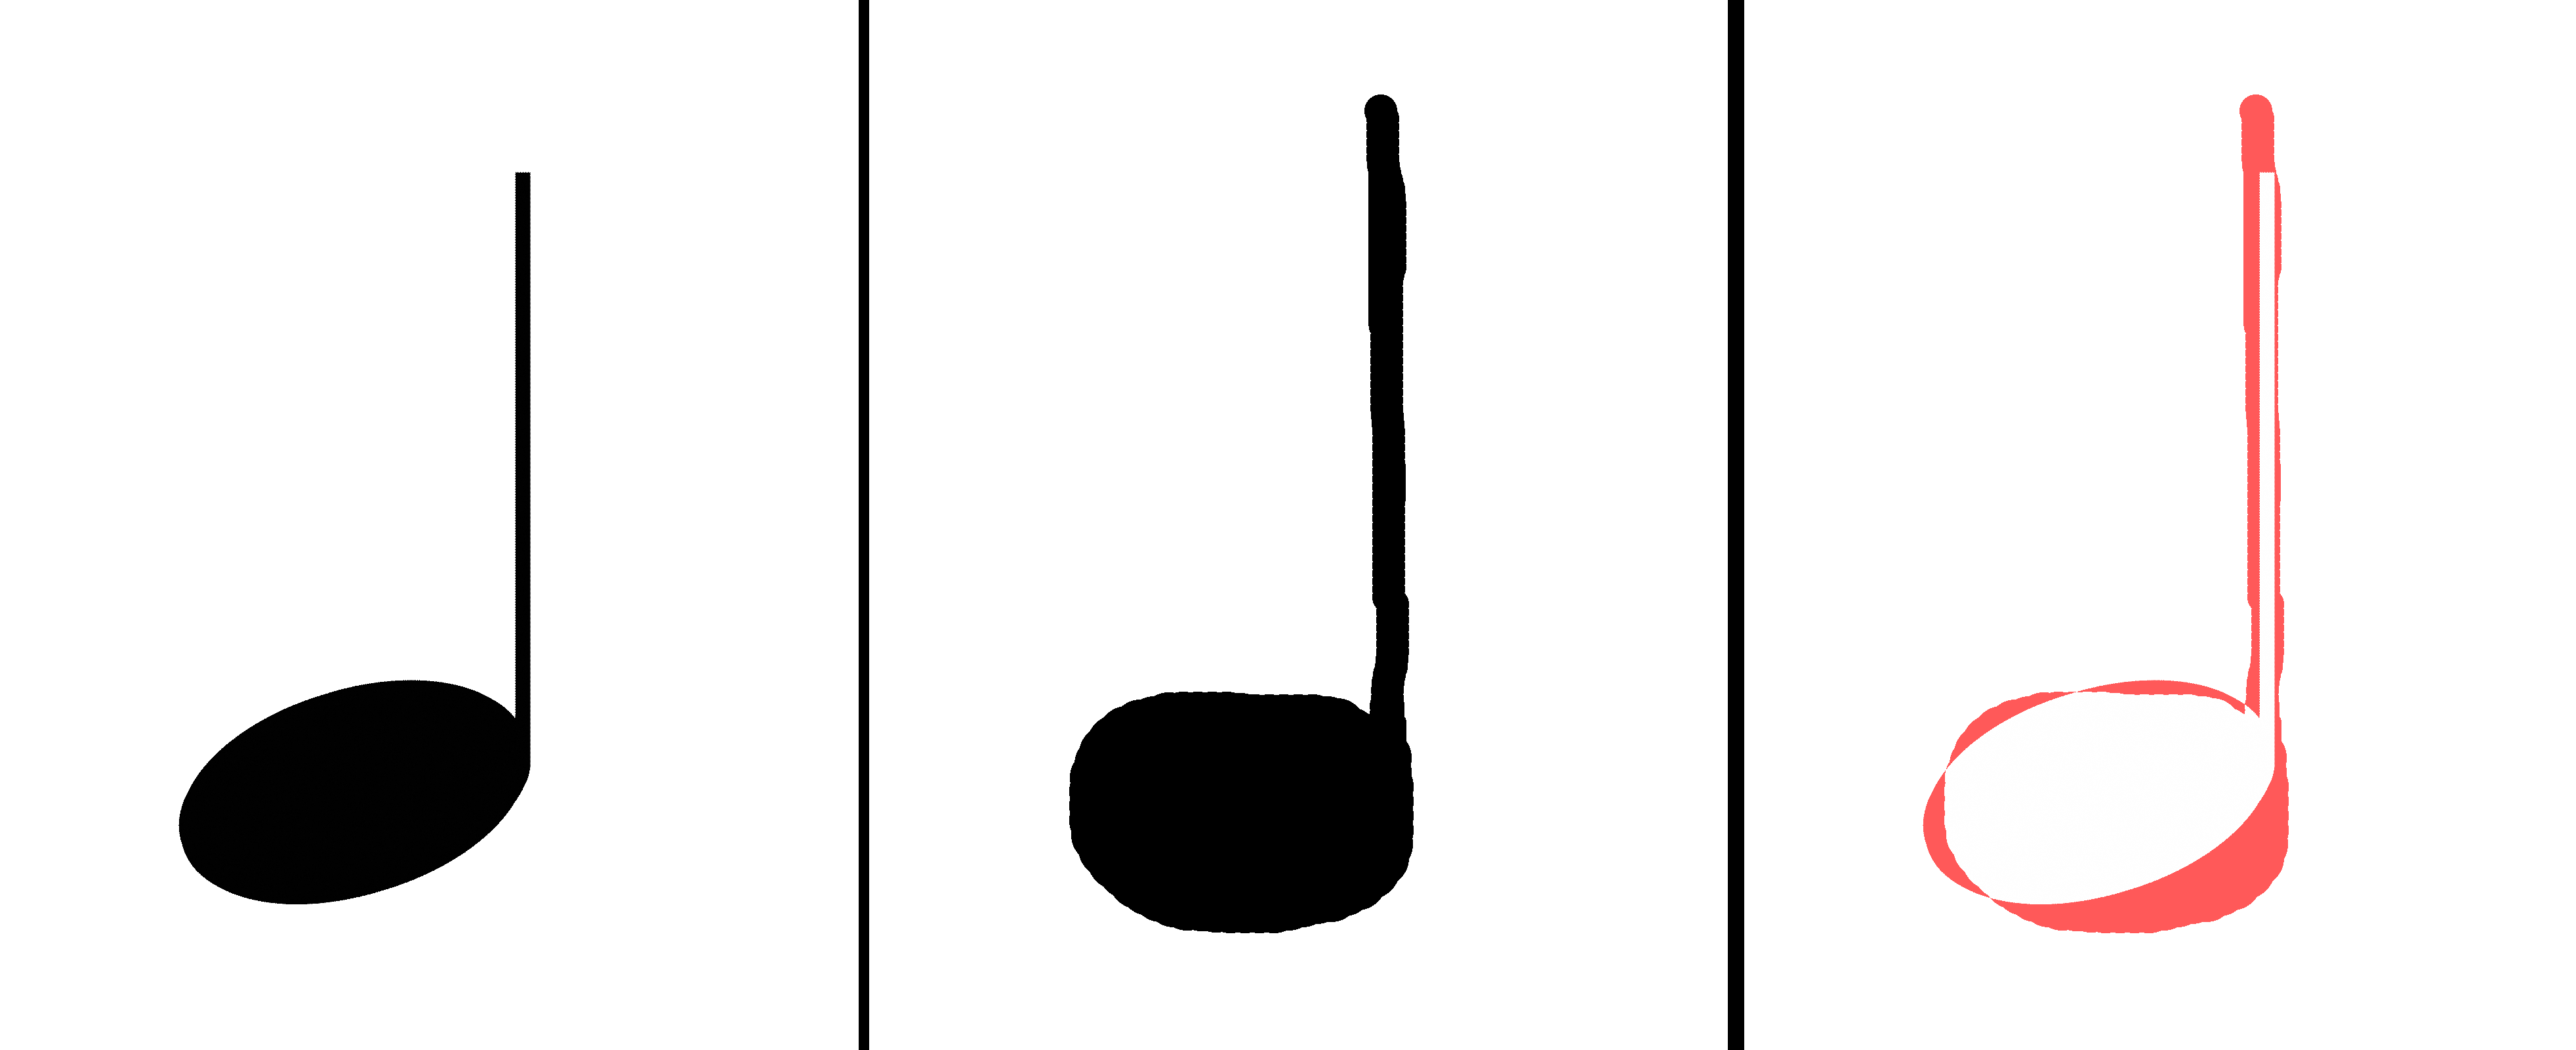
\includegraphics[width=\linewidth]{gfx/crochet-all.png}
  \caption{Highlighting differences between a perfect and a hand-drawn crochet}
  \label{crotchet-diff}
\end{figure}

\todo[inline]{Image Difference: Upside: Very visual, clear what's wrong}
\todo[inline]{Image Difference: Downside: Sensitive to the blob size, means stem errors are less likely to impact the score}

\subsection{Skeletonization}
\label{sec:skeletonization}

Skeletonization is the process of reducing a component in a binary image to a single-pixel wide skeleton. The algorithm used in this project (as defined in \cite{zhang1984fast}) works by making successive passes of the image, removing pixels on object borders. This continues until no more pixels can be removed as in \cref{fig:skeletonization-example}.  The image is correlated with a mask that assigns each pixel a number in the range $[0...255]$ corresponding to each possible pattern of its $8$ neighbouring pixels. A look up table is then used to assign the pixels a value of $0, 1, 2 \text{or} 3$, which are selectively removed during the iterations.

\begin{figure}[H]
  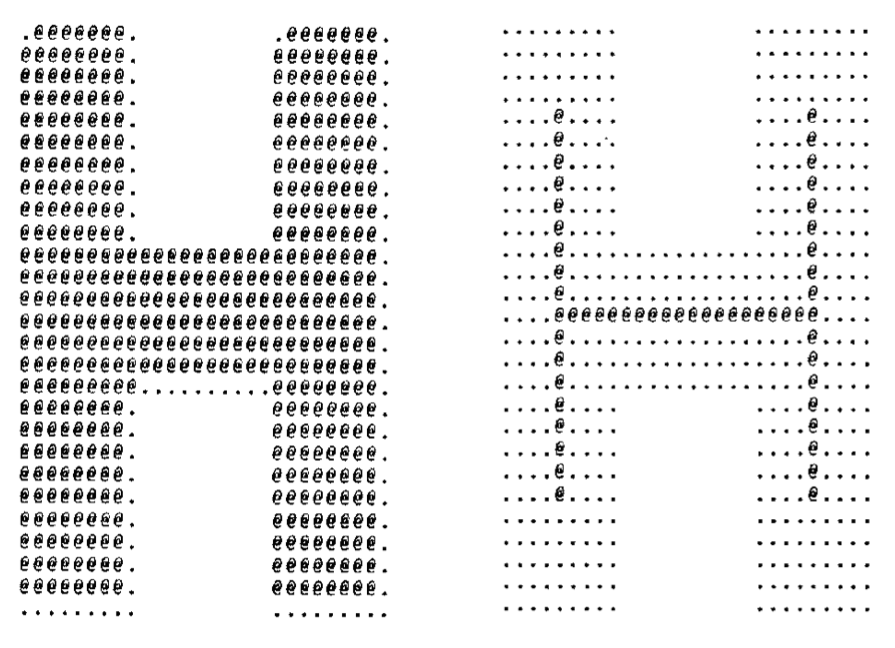
\includegraphics{gfx/skeletonization.png}
  \caption{Results of the skeletonization algorithm from \cite{zhang1984fast}}
  \label{fig:skeletonization-example}
\end{figure}


\subsection{Watershed Segmentation}

\todo[inline,color=red]{Scoring - Watershed Segmentation (for use in heads and islands)}